\documentclass[12pt,a4paper]{article}
\usepackage{listings}
\usepackage{xcolor}

\definecolor{codegreen}{rgb}{0,0.6,0}
\definecolor{codegray}{rgb}{0.5,0.5,0.5}
\definecolor{codepurple}{rgb}{0.58,0,0.82}
\definecolor{backcolour}{rgb}{0.95,0.95,0.92}

\lstdefinestyle{mystyle}{
    % backgroundcolor=\color{backcolour},   
    commentstyle=\color{codegreen},
    keywordstyle=\color{magenta},
    % numberstyle=\tiny\color{codegray},
    stringstyle=\color{codepurple},
    basicstyle=\ttfamily\footnotesize,
    breakatwhitespace=false,         
    breaklines=true,                 
    captionpos=b,                    
    keepspaces=true,                 
    % numbers=left,                    
    % numbersep=5pt,                  
    showspaces=false,                
    showstringspaces=false,
    showtabs=false,                  
    tabsize=2
}

\lstset{style=mystyle}

\usepackage{enumerate}
\usepackage{graphicx}
\graphicspath{ {./images/} }
\usepackage{pgf}
\usepackage{svg}
\usepackage{tikz}
\usepackage{stanli}
\usepackage{afterpage}
\usepackage{multirow}
\usepackage{subfig}
\usepackage{pgfpages}
\usepackage{svg}
\usepackage{rotating}
\usepackage{graphicx,parskip,appendix,float}
\def\@submitdate{\number\the\day\space\space
  \ifcase\the\month\or
  January\or February\or March\or April\or May\or June\or
  July\or August\or September\or October\or November\or December\fi
  \space \number\the\year}

\pgfpagesdeclarelayout{boxed}
{
    \edef\pgfpageoptionborder{0pt}
}
% Border Settings
{
    \pgfpagesphysicalpageoptions
    {%
        logical pages=1,%
    }
    \pgfpageslogicalpageoptions{1}
    {
        border code=\pgfsetlinewidth{0.5pt}\pgfstroke,%
        border shrink=\pgfpageoptionborder,%
        resized width=.9\pgfphysicalwidth,%
        resized height=.9\pgfphysicalheight,%
        center=\pgfpoint{.5\pgfphysicalwidth}{.5\pgfphysicalheight}%
    }%
}

\pgfpagesuselayout{boxed}

\usepackage[english]{babel}

\usepackage[a4paper,top=1.5cm,bottom=1.5cm,left=1.5cm,right=1.5cm,marginparwidth=1cm]{geometry}

% Useful packages
\usepackage{amsmath}
\usepackage{graphicx}
\usepackage[colorlinks=true, allcolors=blue]{hyperref}

\title{}
\author{}
\date{}

\begin{document}
	
\newcommand{\subf}[2]{%
    {\small\begin{tabular}[t]{@{}c@{}}
            #1\\#1
    \end{tabular}}%
}

\begin{titlepage}
    \begin{center}
        \vspace{1cm}		
        \Huge
        \textbf{EN3160 - Image Processing and Machine Vision}

        \vspace{0.5cm}
        %\Huge
        {\LARGE Assignment 01 on Intensity Transformations and Neighborhood
Filtering}
        \vspace{1cm}
        \large			
        \vspace{0.5cm}
        \LARGE			
        \vspace{3cm}
        
        \textbf{}
        
\includegraphics[width=0.3\textwidth]{university.png}\\
        {\Large University of Moratuwa}
        \\
        {\Large Sri Lanka}
        \vfill			
        \vspace{0.4cm}
        \Large
    \end{center}
    
    \Large
    \vspace{1cm}
    \begin{tabbing}
        \hspace*{11em}\= \hspace*{4em} \= \kill % set the tabbings
        %\> Group \> : Group D \\
        \> Name\> :  Abithan A.\\
        \> Reg No\>:  210019E \\
    \end{tabbing}
    % \begin{figure}[!b]
    % \begin{center}
    % Copyright \copyright\; 2011 Dan Eiblum\\
    % All rights reserved\\
    
    % ISBN: 978-1-4610-9314-5\\
    % \textbf{Library of Congress Control Number: 2011905974}
    % \end{center}
    % \end{figure}
     \centering
    % \@submitdate \\
    \href{https://github.com/Abithan07/-Intensity-Transformations-and-Neighborhood-Filtering/tree/main}{\normalsize{github.com/Abithan07/-Intensity-Transformations-and-Neighborhood-Filtering}}
    
    \vspace{8mm}
    
\includegraphics[height=10mm]{ent.png}
\end{titlepage}

%%%%%%%%%%%%%%%%%%%%%%%%%%%%%%%%%%%%%%%%%%%%%%%%%%%%%%%%%%%%%%%%%%%%%%%%%%%	

\section{Implement the intensity transformation}

    \begin{figure}[H]
        \centering
        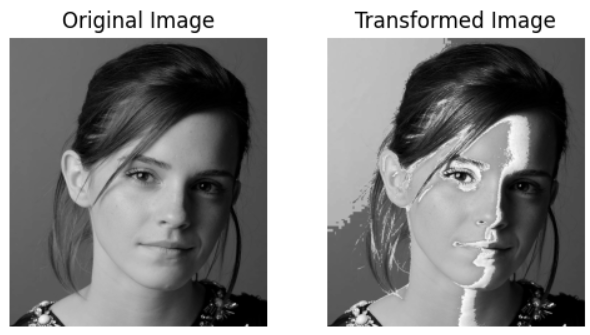
\includegraphics[width=0.5\linewidth]{images/Screenshots/1.png}
        \caption{Original and Intensity transformed images}
        \label{fig:enter-label}
    \end{figure}

    % \begin{itemize}
    %     \item Code used:
    % \end{itemize}
    
    % \lstinputlisting[language=python]{Code/1.py}
    

\section{ brain proton density image intensity transformations}

    \begin{figure}[H]
        \centering
        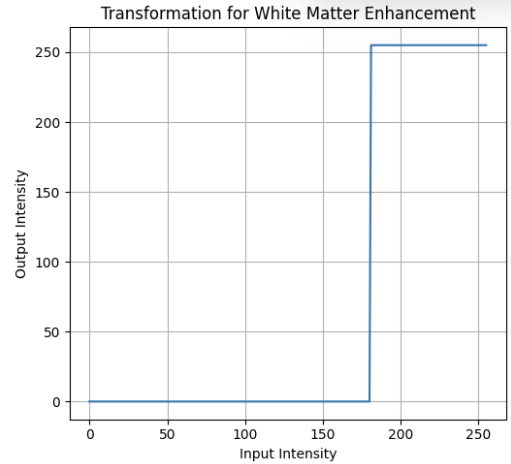
\includegraphics[width=0.3\linewidth]{images/Screenshots/2_1.png}
        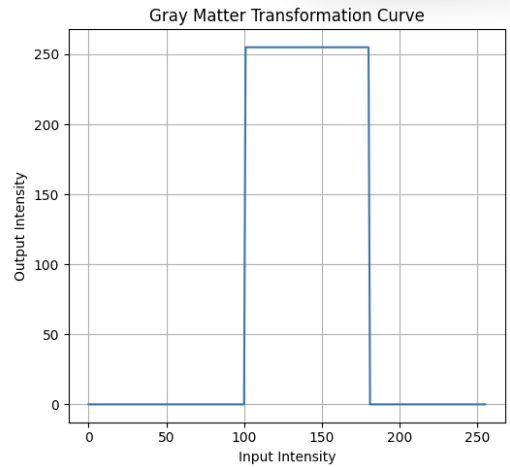
\includegraphics[width=0.3\linewidth]{images/Screenshots/2_2.png}
        \caption{White and gray matter Intensity transformation plots}
        \label{fig:enter-label}
    \end{figure}




\section{Gamma correction}
    \begin{figure}[H]
        \centering
        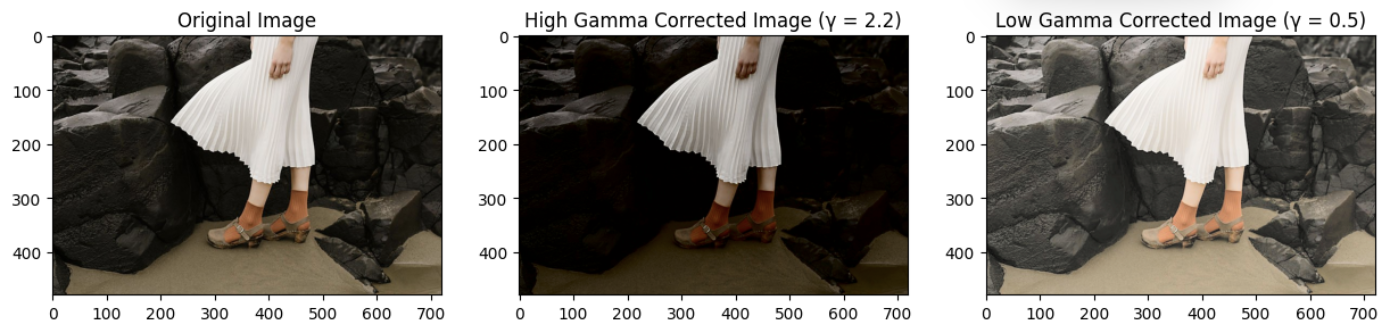
\includegraphics[width=0.85\linewidth]{images/Screenshots/3_1.png}
        \caption{Original and gamma corrected images}
        \label{fig:enter-label}
    \end{figure}

    \begin{figure}[H]
        \centering
        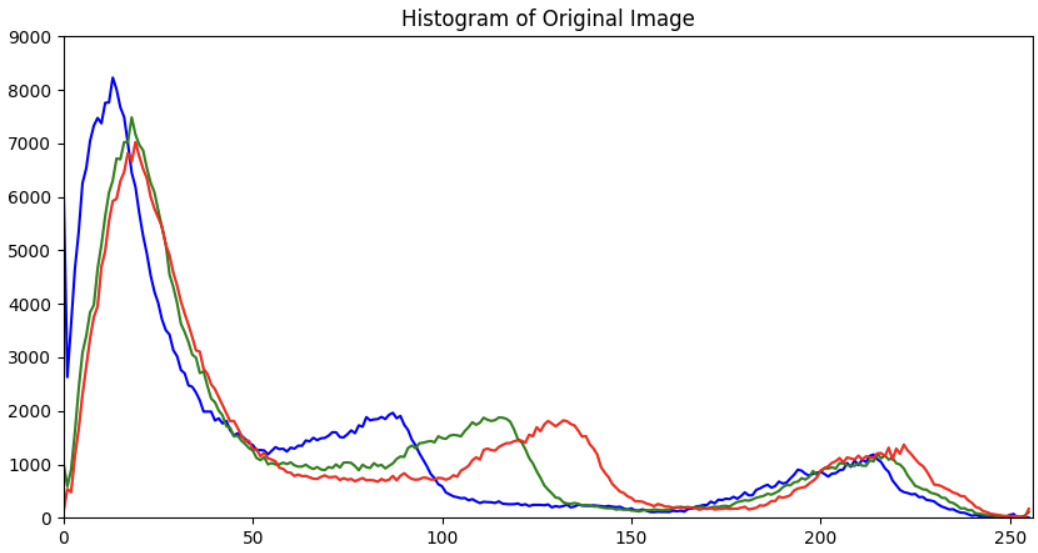
\includegraphics[width=0.3\linewidth]{images/Screenshots/3_2.png}
        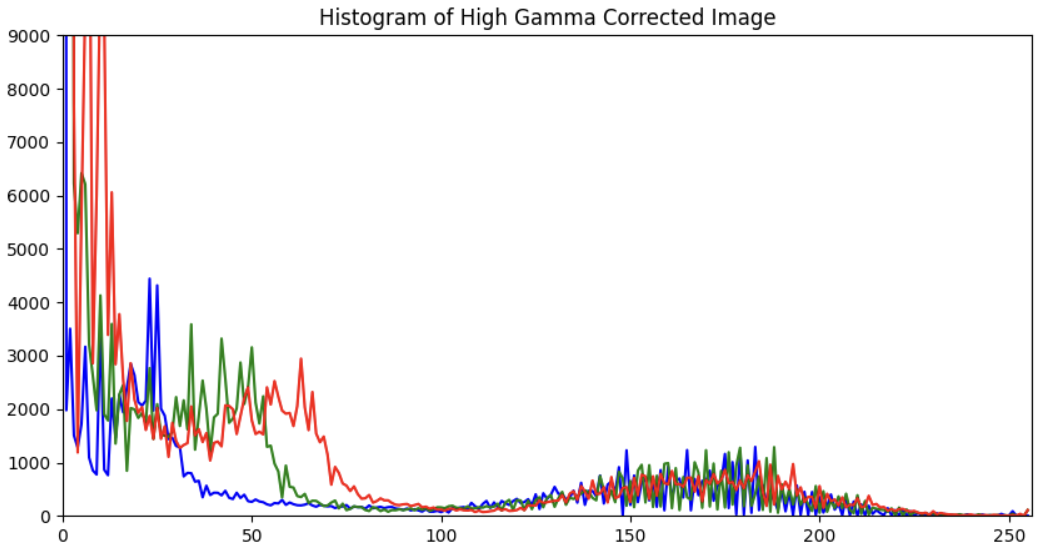
\includegraphics[width=0.3\linewidth]{images/Screenshots/3_3.png}
        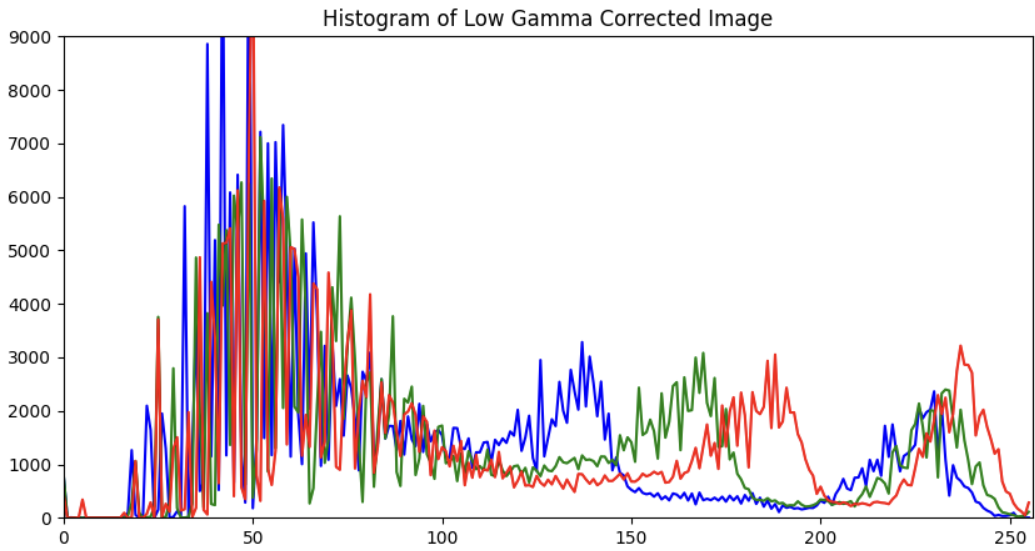
\includegraphics[width=0.3\linewidth]{images/Screenshots/3_4.png}
        \caption{Histograms of Original and gamma corrected images}
        \label{fig:enter-label}
    \end{figure}

    % \begin{itemize}
    %     \item Code used:
    % \end{itemize}
    
    % \lstinputlisting[language=python]{Code/3.py}

\section{Increasing the vibrance of a photograph}

    \begin{enumerate}
        \item[a.] Split the image into hue, saturation, and value planes.

    \begin{figure}[H]
        \centering
        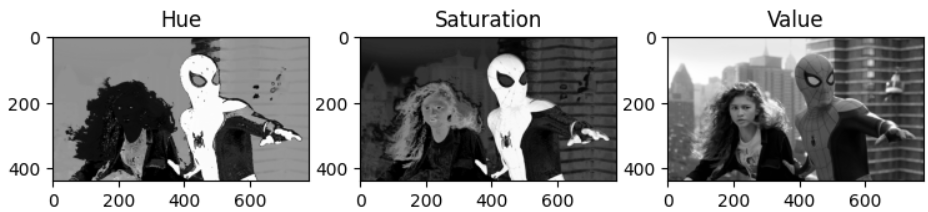
\includegraphics[width=0.85\linewidth]{images/Screenshots/4a.png}
        \caption{Splited hsv planes}
        \label{fig:enter-label}
    \end{figure}
    
    % \begin{itemize}
    %     \item Code Snippet:
    % \end{itemize}
    
    % \lstinputlisting[language=python]{Code/4a.py}

    
    \item[b.] Apply the aforementioned intensity transformation to the saturation plane.

    \begin{itemize}
        \item Code Snippet:
    \end{itemize}
    
    \lstinputlisting[language=python]{Code/4b.py}

    
    \item[c.] Adjust 'a' to get a visually pleasing output.
    \begin{figure}[H]
        \centering
        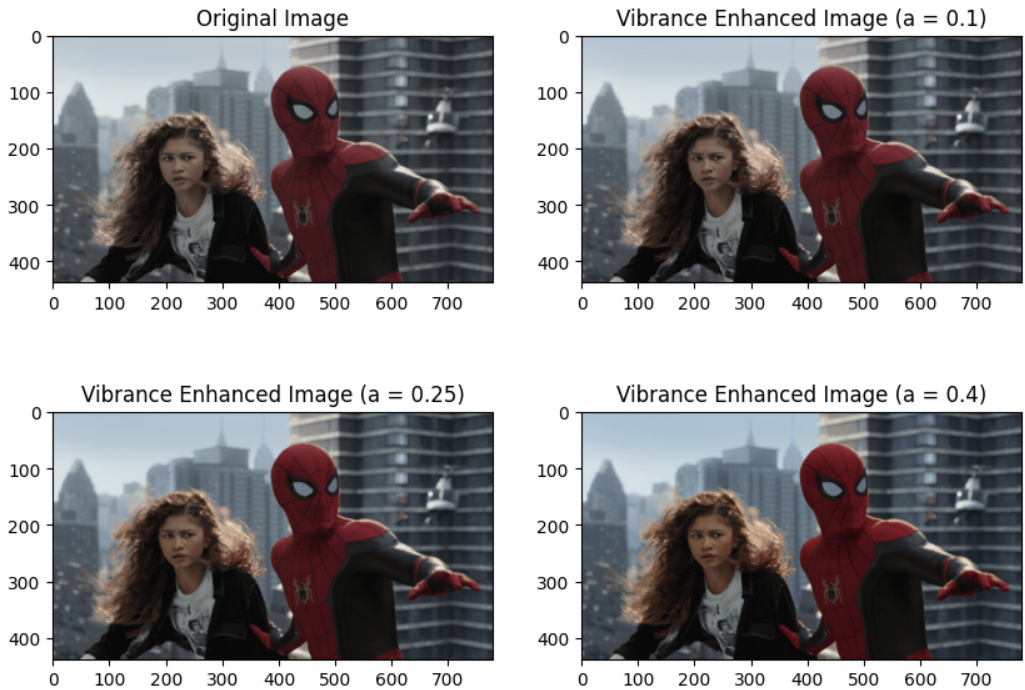
\includegraphics[width=0.45\linewidth]{images/Screenshots/4c1.png}
        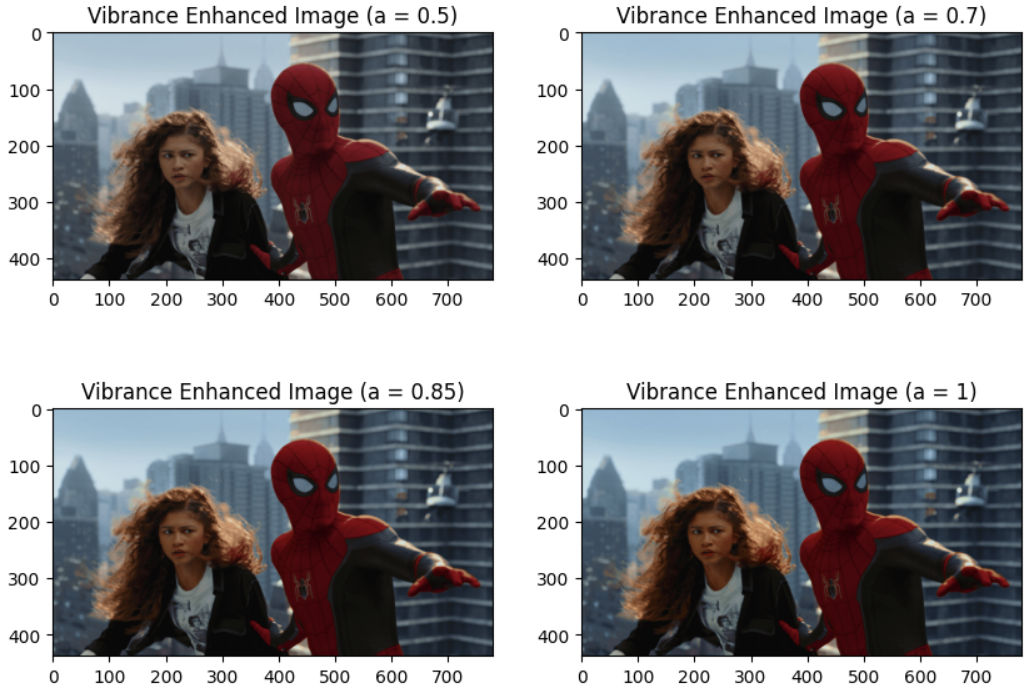
\includegraphics[width=0.45\linewidth]{images/Screenshots/4c2.png}
        \caption{Vibrance adjusted images with different a values}
        \label{fig:enter-label}
    \end{figure}    

    
    \item[d.] Recombine the three planes.
    \begin{itemize}
        \item Code Snippet:
    \end{itemize}
    
    \lstinputlisting[language=python]{Code/4d.py}

    
    \item[e.] Display the original image, vibrance-enhanced image, and the intensity transformation

    \begin{figure}[H]
        \centering
        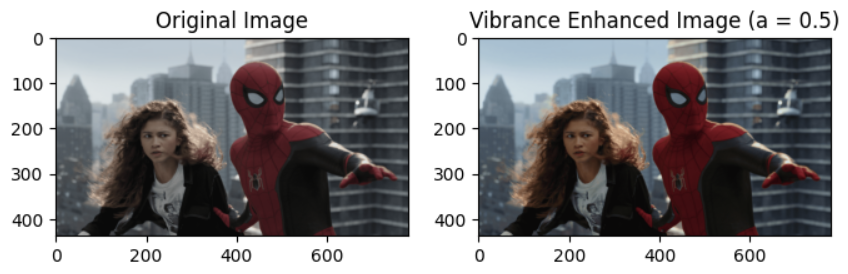
\includegraphics[width=0.6\linewidth]{images/Screenshots/4e1.png}
        \caption{original and vibrance-enhanced images for a=0.5}
        \label{fig:enter-label}
    \end{figure}

    \begin{figure}[H]
        \centering
        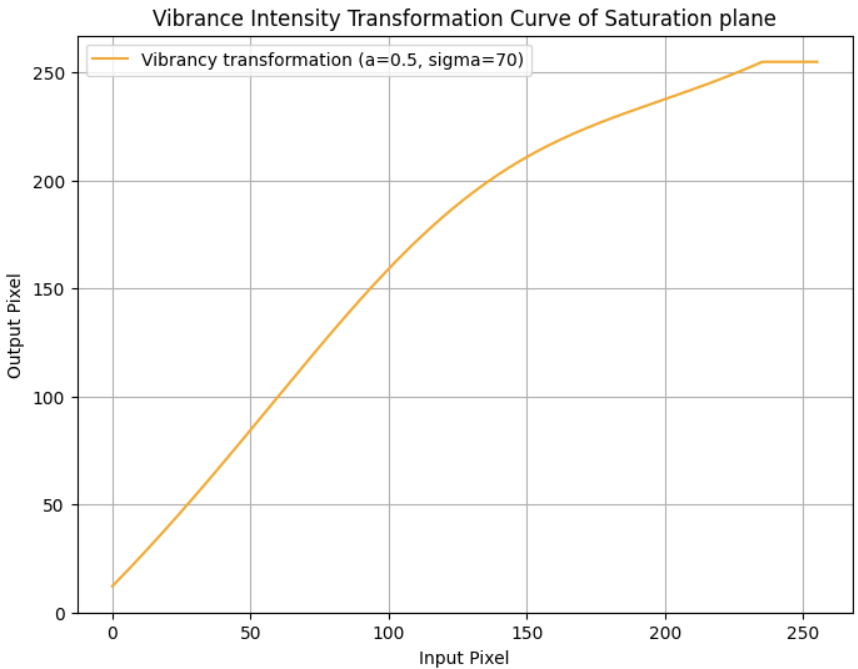
\includegraphics[width=0.3\linewidth]{images/Screenshots/4e2.png}
        \caption{Vibrance intensity transformation curve}
        \label{fig:enter-label}
    \end{figure}
    

    % \begin{itemize}
    %     \item Code Snippet:
    % \end{itemize}
    
    % \lstinputlisting[language=python]{Code/4d.py}
    
    \end{enumerate}

\section{Custom function to carry out histogram equalization}

    \begin{figure}[H]
        \centering
        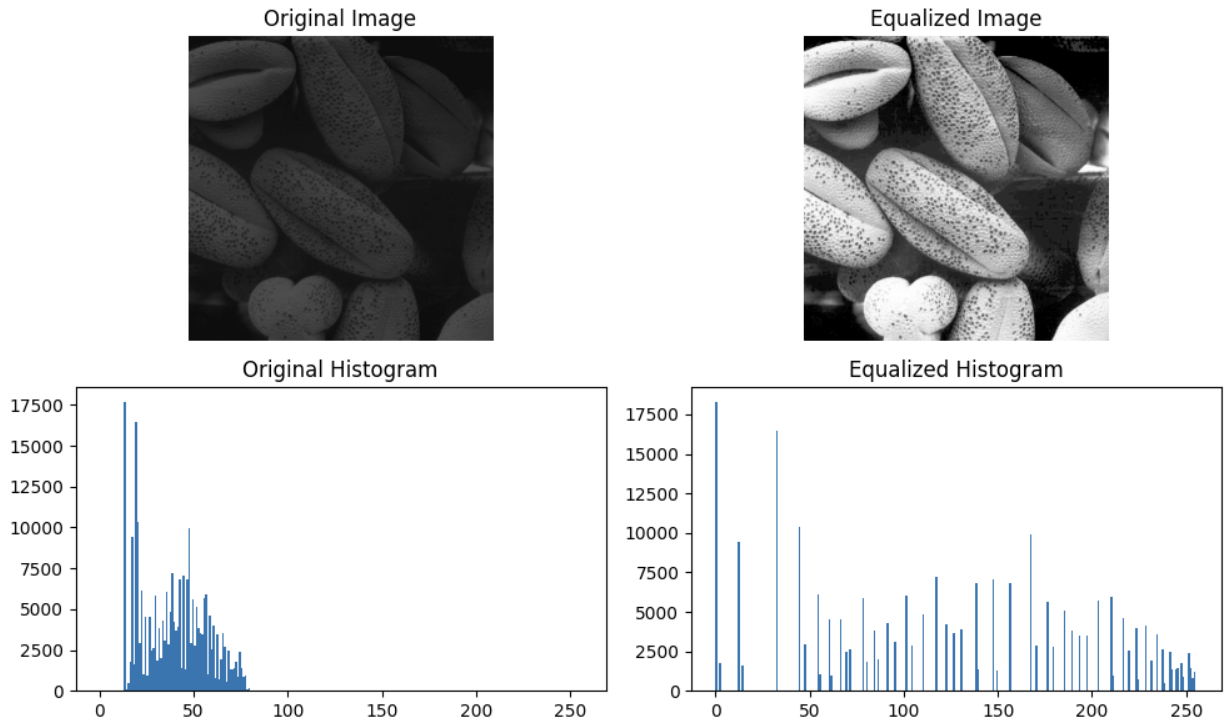
\includegraphics[width=0.6\linewidth]{images/Screenshots/5.png}
        \caption{Normal and equalized images with histograms}
        \label{fig:enter-label}
    \end{figure}

    \begin{itemize}
        \item Code Snippet:
    \end{itemize}

    \lstinputlisting[language=python]{Code/5.py}

\section{Image with a histogram equalized foreground}

    \begin{enumerate}
        \item[a.] split it into hue, saturation, and values and display these planes in grayscale.
    

    \begin{figure}[H]
        \centering
        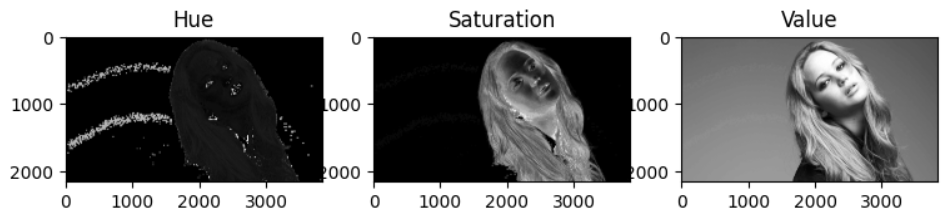
\includegraphics[width=0.8\linewidth]{images/Screenshots/6a.png}
        \caption{Splited hsv planes}
        \label{fig:enter-label}
    \end{figure}

    \item[b.] Select the appropriate plane to threshold in extract the foreground mask.

    \begin{itemize}
        \item Saturation plane
    \end{itemize}
    
    \begin{figure}[H]
        \centering
        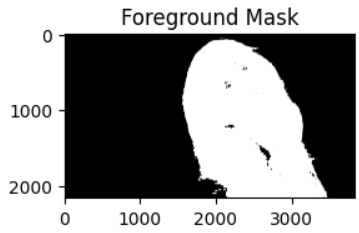
\includegraphics[width=0.3\linewidth]{images/Screenshots/6b.png}
        \caption{Foreground Mask}
        \label{fig:enter-label}
    \end{figure}

    \item[c.] Obtain the foreground only and compute the histogram.

    \begin{figure}[H]
        \centering
        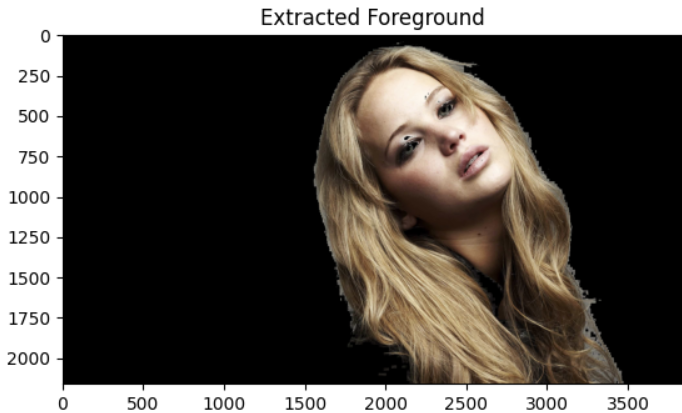
\includegraphics[width=0.3\linewidth]{images/Screenshots/6c1.png}
        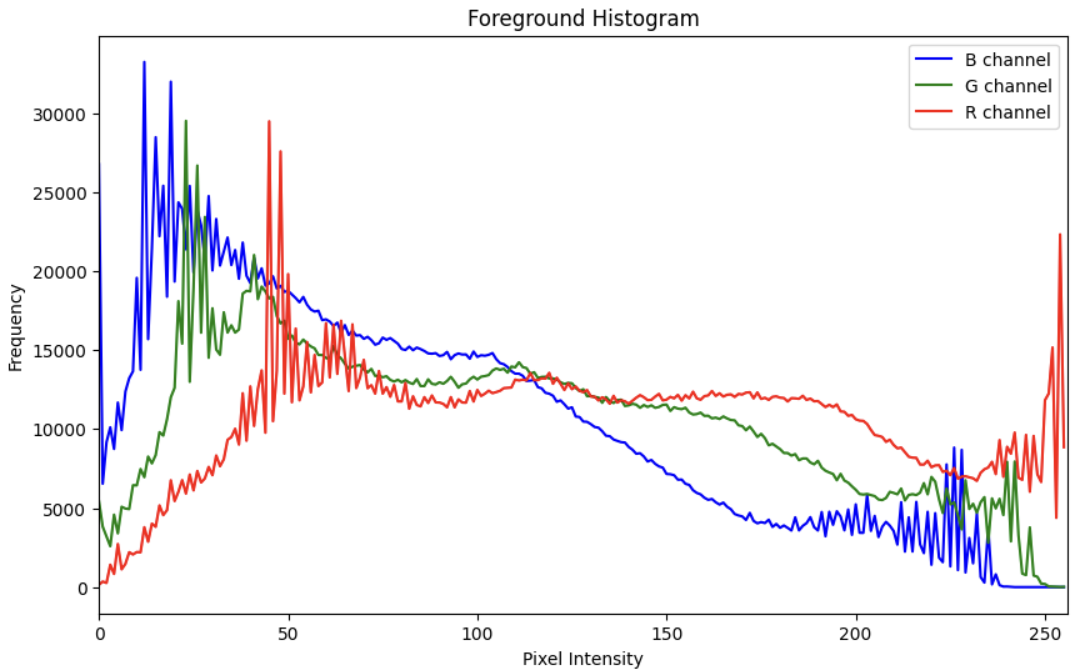
\includegraphics[width=0.3\linewidth]{images/Screenshots/6c2.png}
        \caption{Foreground and it's histogram}
        \label{fig:enter-label}
    \end{figure}

    \item[d.] Obtain the cumulative sum of the histogram.
    \begin{figure}[H]
        \centering
        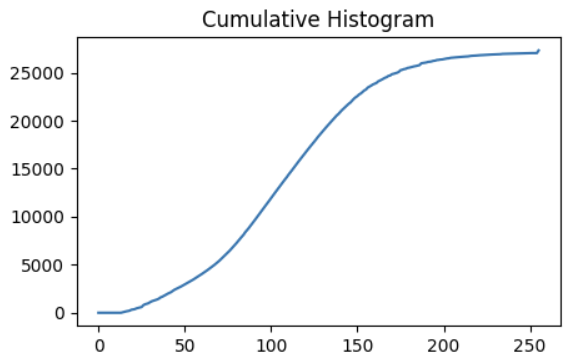
\includegraphics[width=0.3\linewidth]{images/Screenshots/6d.png}
        \caption{cumulative sum of the histogram}
        \label{fig:enter-label}
    \end{figure}

    \item[e.] Histogram-equalize the foreground.

    \begin{figure}[H]
        \centering
        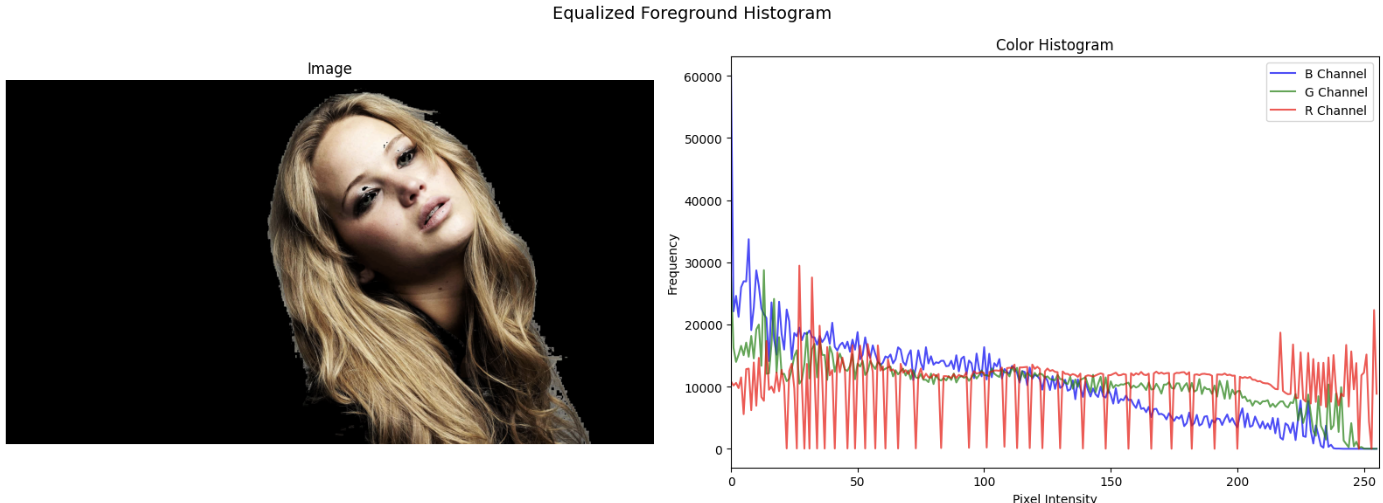
\includegraphics[width=0.6\linewidth]{images/Screenshots/6e.png}
        \caption{Equalized foreground with Histogram}
        \label{fig:enter-label}
    \end{figure}

    \item[f.] Extract the background and add with the histogram equalized foreground.

    \begin{figure}[H]
        \centering
        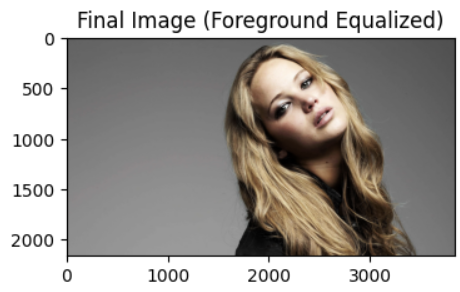
\includegraphics[width=0.3\linewidth]{images/Screenshots/6f.png}
        \caption{Final Image}
        \label{fig:enter-label}
    \end{figure}

\end{enumerate}

\section{Filtering with the Sobel operator}

    \begin{enumerate}
        \item[a.] Using the existing filter2D to Sobel filter the image.
        \lstinputlisting[language=python]{Code/7a.py}
        
        \item[b.] Write your own code to Sobel filter the image
        \lstinputlisting[language=python]{Code/7b.py}
        
        \item[c.] Using the property carry out Sobel filtering. 
        \lstinputlisting[language=python]{Code/7c.py}
    \end{enumerate}

\section{Zooming images}

    \begin{enumerate}
        \item[a.] nearest-neighbor
        \lstinputlisting[language=python]{Code/8a.py}

        \item[b.] bilinear interpolation
        \lstinputlisting[language=python]{Code/8b.py}
        
    \end{enumerate}

\section{Background Blur}

    \begin{enumerate}
        \item[a.] Use grabCut to segment the image.

            % \begin{itemize}
            %     \item Code Snippet:
            % \end{itemize}
        
            % \lstinputlisting[language=python]{Code/9a.py}
        
            \begin{figure}[H]
                \centering
                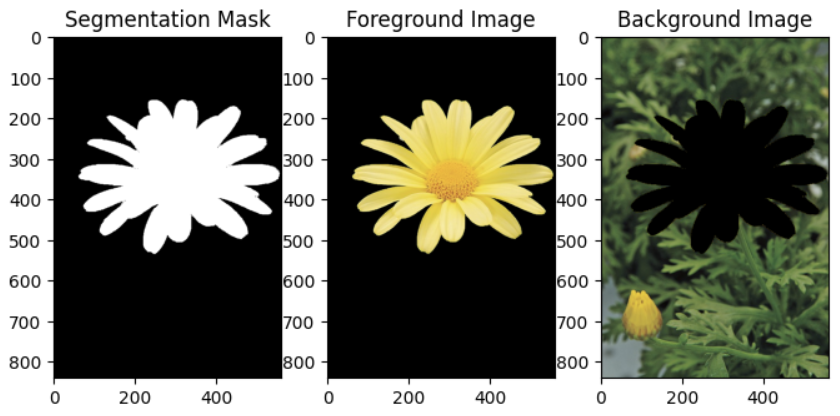
\includegraphics[width=0.5\linewidth]{images/Screenshots/9a.png}
                \caption{Segmentation mask, foreground, and background images}
                \label{fig:enter-label}
            \end{figure}

    \item[b.]  Produce an enhanced image with a substantially blurred background.

        % \lstinputlisting[language=python]{Code/9b.py}
    
        \begin{figure}[H]
            \centering
            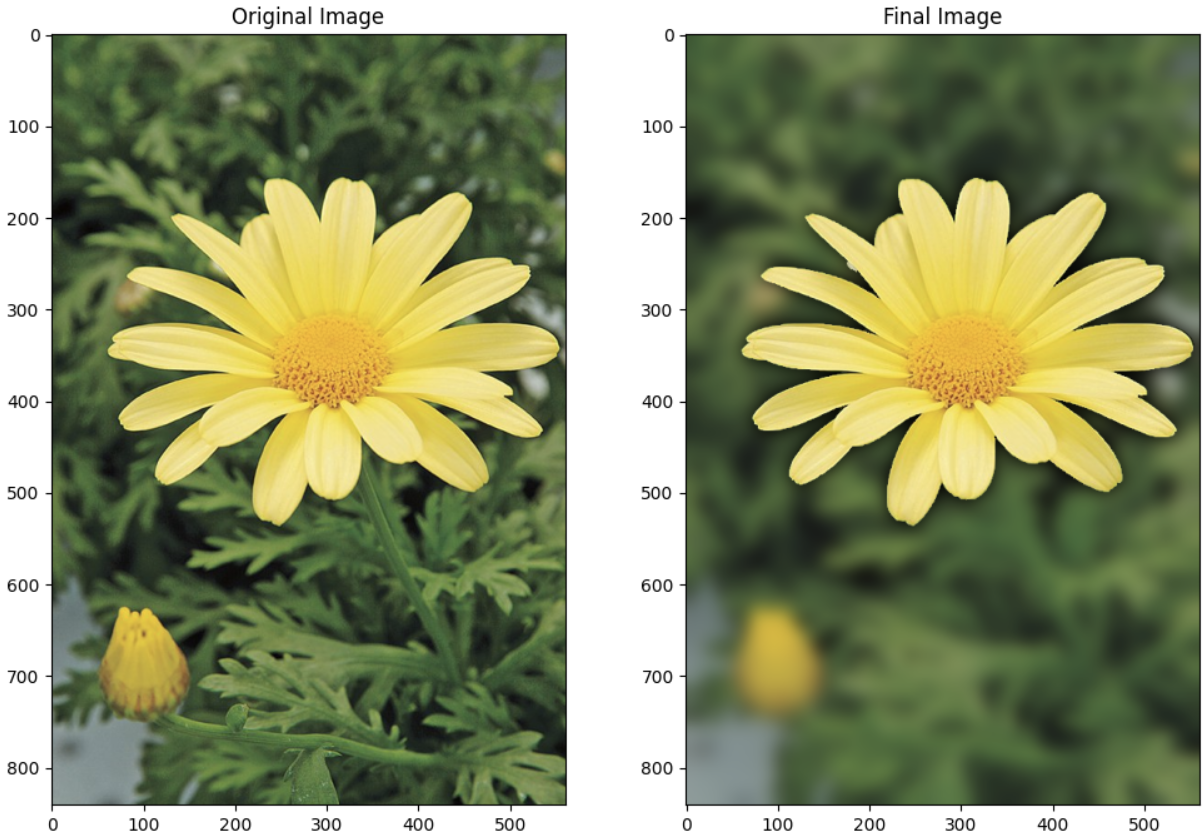
\includegraphics[width=0.4\linewidth]{images/Screenshots/9b.png}
            \caption{Original and Final images}
            \label{fig:enter-label}
        \end{figure}

    \item[c.] Why is the background just beyond the edge of the flower quite dark in the enhanced image?

    \begin{itemize}
        \item The Gaussian blur kernel uses neighboring dark pixels to compute the new pixel value, so they also influence the filtering.
        
    \end{itemize}
        
    
    \end{enumerate}
    


\end{document}
